\documentclass[tikz,border=4pt]{standalone}

\usepackage{amsmath}
\usepackage{amssymb}
\usepackage{xcolor}
\usepackage{tikz}


\usetikzlibrary{
    arrows,
    arrows.meta,
    automata,
    backgrounds,
    calc,
    decorations.pathreplacing,
    fit,
    matrix,
    positioning,
    shapes,
    shapes.arrows,
    shapes.geometric,
    shapes.multipart
}



\tikzset{
  start/.style={
    rectangle,
    rounded corners,
    minimum width=3.5cm,
    minimum height=1cm,
    text centered,
    text width=3cm,
    draw=black,
    fill=green!20
  },
  stop/.style={
    rectangle,
    rounded corners,
    minimum width=3cm,
    minimum height=1cm,
    text centered,
    text width=2.5cm,
    draw=black,
    fill=red!20
  },
  decision/.style={
    diamond,
    aspect=2,
    minimum width=3cm,
    minimum height=1.2cm,
    text centered,
    text width=2.5cm,
    inner sep=1pt,
    draw=black,
    fill=yellow!20
  },
  process/.style={
    rectangle,
    minimum width=3cm,
    minimum height=1cm,
    text centered,
    text width=2.7cm,
    draw=black,
    fill=blue!10
  },
  arrow/.style={
    thick,
    -{Stealth}
  }
}


\usetikzlibrary{
  arrows.meta,
  positioning,
  shapes.geometric
}

\tikzset{
  start/.style={
    rectangle,
    rounded corners,
    minimum width=3.5cm,
    minimum height=1cm,
    text centered,
    text width=3cm,
    draw=black,
    fill=green!20
  },
  stop/.style={
    rectangle,
    rounded corners,
    minimum width=3cm,
    minimum height=1cm,
    text centered,
    text width=2.5cm,
    draw=black,
    fill=red!20
  },
  decision/.style={
    diamond,
    aspect=2,
    minimum width=3cm,
    minimum height=1.2cm,
    text centered,
    text width=2.5cm,
    inner sep=1pt,
    draw=black,
    fill=yellow!20
  },
  io/.style={
    trapezium,
    trapezium left angle=70,
    trapezium right angle=110,
    minimum width=3.5cm,
    minimum height=1cm,
    text centered,
    text width=3cm,
    draw=black,
    fill=blue!20
  },
  arrow/.style={
    thick,
    -{Stealth}
  }
}

\input{../jpk.inc}


\begin{document}

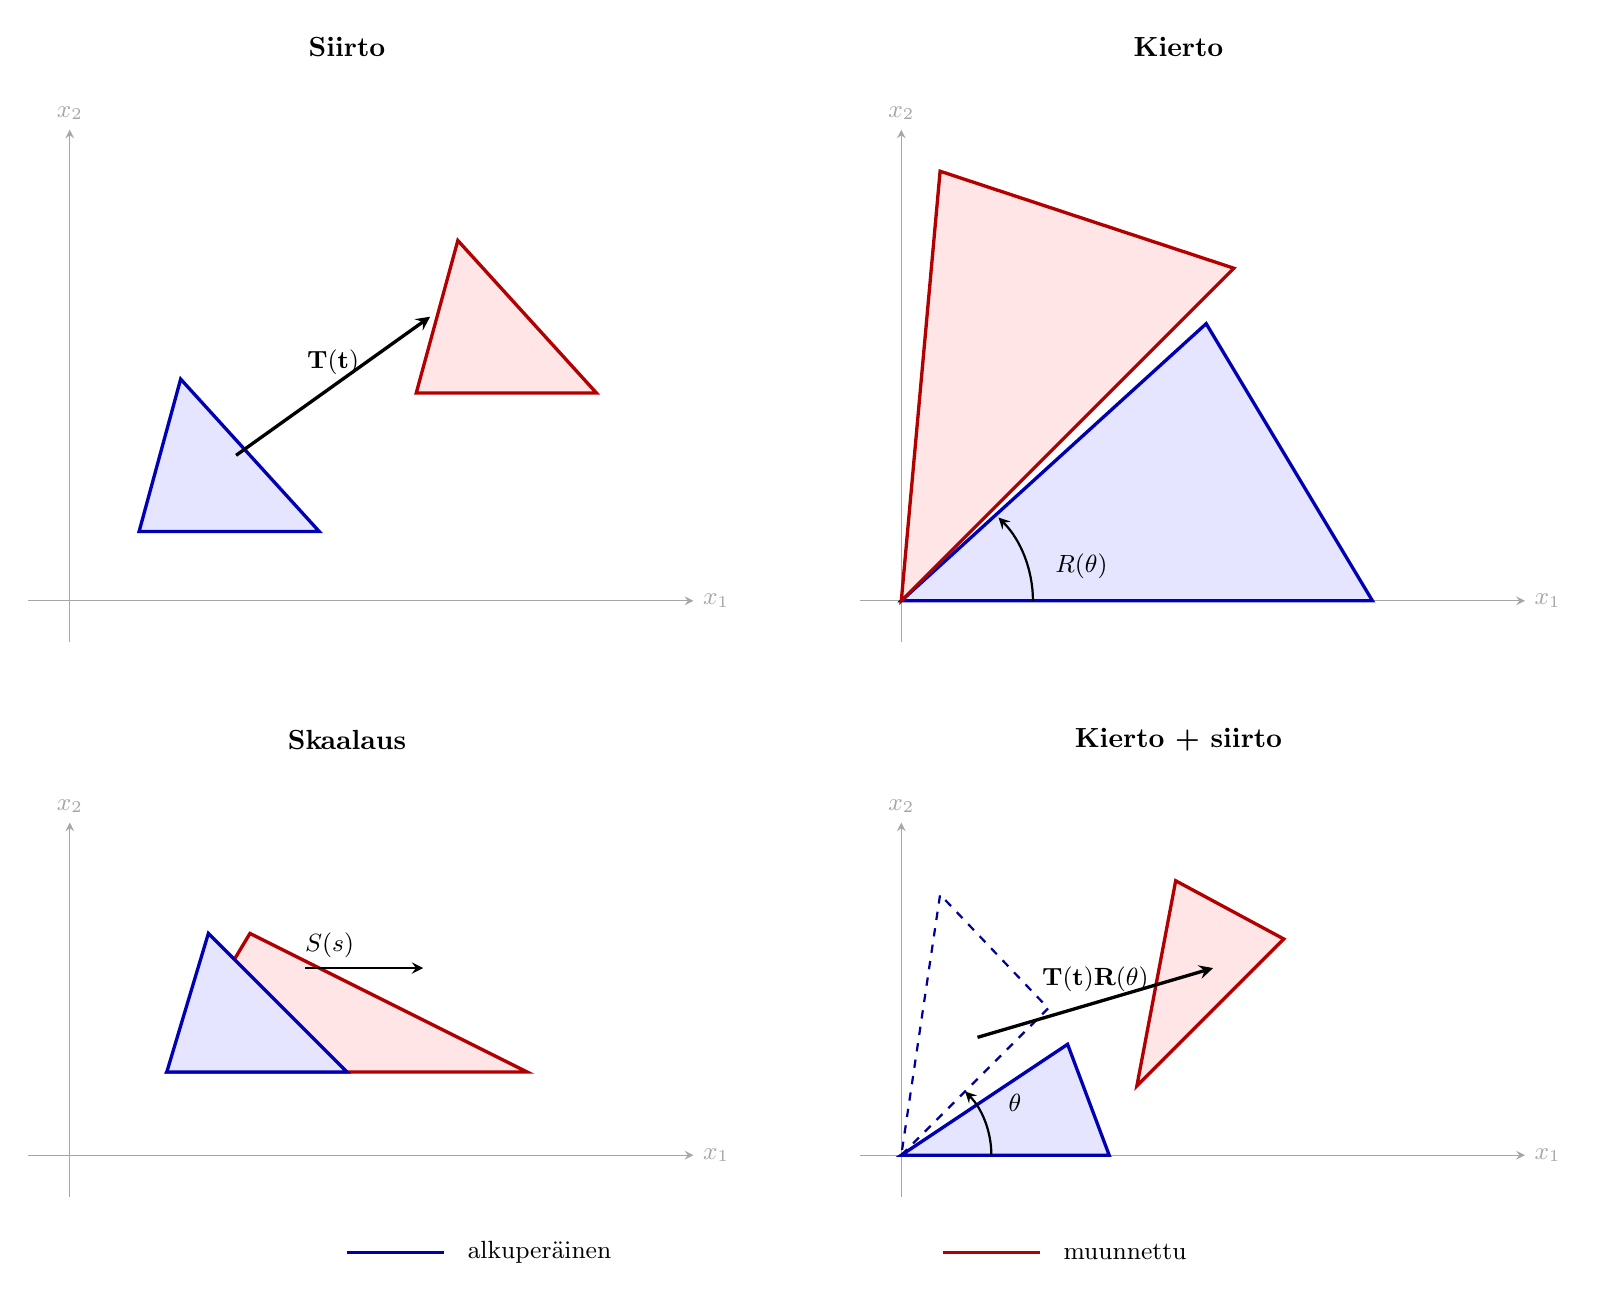
\begin{tikzpicture}[
        scale=1.76,
        >=stealth,
        font=\small,
        axis/.style={->, gray!70},
        original/.style={blue!70!black, very thick, fill=blue!10},
        transformed/.style={red!70!black, very thick, fill=red!10}
        ]
        
\begin{scope}[xshift=0cm,yshift=4cm]
          
          \node[font=\bfseries] at (2,4.0) {Siirto};
          
          \draw[axis] (-0.3,0) -- (4.5,0) node[right] {$x_1$};
          \draw[axis] (0,-0.3) -- (0,3.4) node[above] {$x_2$};
          
\draw[original]
          (0.5,0.5) -- (1.8,0.5) -- (0.8,1.6) -- cycle;
          
\draw[transformed]
          (2.5,1.5) -- (3.8,1.5) -- (2.8,2.6) -- cycle;
          
\draw[->, very thick]
          (1.2,1.05) -- (2.6,2.05)
          node[midway, above] {$\mathbf{T(t)}$};          
        \end{scope}
        
        
\begin{scope}[xshift=6cm,yshift=4cm]
          
          \node[font=\bfseries] at (2,4.0) {Kierto};
          
          \draw[axis] (-0.3,0) -- (4.5,0) node[right] {$x_1$};
          \draw[axis] (0,-0.3) -- (0,3.4) node[above] {$x_2$};
          


\draw[original]
          (0,0) -- (3.4,0) -- (2.2,2.0) -- cycle;


\draw[transformed]
          (0,0) -- (2.4,2.4) -- (0.28,3.1) -- cycle;


\draw[->, thick]
          (0.95,0)
arc[start angle=0,end angle=45,radius=0.85];
          
          \node at (1.3,0.25) {$\V{R}(\theta)$};
          
        \end{scope}
        
        
\begin{scope}[xshift=0cm,yshift=0cm]
          
          \node[font=\bfseries] at (2,3.0) {Skaalaus};
          
          \draw[axis] (-0.3,0) -- (4.5,0) node[right] {$x_1$};
          \draw[axis] (0,-0.3) -- (0,2.4) node[above] {$x_2$};
          
          
\draw[transformed]
          (0.7,0.6) -- (3.3,0.6) -- (1.3,1.6) -- cycle;
          
\draw[original]
          (0.7,0.6) -- (2.0,0.6) -- (1.0,1.6) -- cycle;

\draw[->, thick]
          (1.7,1.35) -- (2.55,1.35)
          node[midway, above left] {$\V{S(s)}$};
          
        \end{scope}
        
        
\begin{scope}[xshift=6cm,yshift=0cm]
          
          \node[font=\bfseries] at (2,3.0) {Kierto + siirto};
          
          \draw[axis] (-0.3,0) -- (4.5,0) node[right] {$x_1$};
          \draw[axis] (0,-0.3) -- (0,2.4) node[above] {$x_2$};
          
\draw[original]
          (0,0) -- (1.5,0) -- (1.2,0.8) -- cycle;


\draw[blue!60!black, thick, dashed]
          (0,0) -- (1.06,1.06) -- (0.28,1.88) -- cycle;


\draw[transformed]
          (1.7,0.5) -- (2.76,1.56) -- (1.98,1.98) -- cycle;


\draw[->, thick]
          (0.65,0)
arc[start angle=0,end angle=45,radius=0.65];
          
          \node at (0.82,0.38) {$\theta$};
          
\draw[->, very thick]
          (0.55,0.85) -- (2.25,1.35)
          node[midway, above] {$\mathbf{T(t)R}(\theta)$};
          
        \end{scope}
        
        


        \draw[original] (2.0,-0.7) -- (2.7,-0.7);
        \node[right] at (2.8,-0.7) {alkuperäinen};
        
        \draw[transformed] (6.3,-0.7) -- (7.0,-0.7);
        \node[right] at (7.1,-0.7) {muunnettu};
        
      \end{tikzpicture}

\end{document}
